\documentclass[conference]{IEEEtran}
\usepackage[T1]{fontenc}
\usepackage{cite}
\usepackage{amsmath}
\usepackage{graphicx}
\usepackage{booktabs}
\usepackage{multirow}
\usepackage{xcolor}
\usepackage[hidelinks]{hyperref}
\usepackage{xurl}
\usepackage{tikz}
\usetikzlibrary{positioning,arrows.meta,fit}
% Generated by paper/make_numbers.py from results/; do not edit by hand.
\newcommand{\CensusSample}{2{,}000}  % results/census/phase2/rq1.json
\newcommand{\DriftPkgs}{731/2{,}000}  % results/census/phase2/rq1.json
\newcommand{\DriftPkgsP}{36.5\%}  % results/census/phase2/rq1.json
\newcommand{\DriftPkgsCI}{[34.5, 38.7]}  % results/census/phase2/rq1.json
\newcommand{\DriftWinRel}{731/1{,}239}  % results/census/phase2/rq1.json
\newcommand{\DriftWinRelP}{59.0\%}  % results/census/phase2/rq1.json
\newcommand{\DriftWinRelCI}{[56.2, 61.7]}  % results/census/phase2/rq1.json
\newcommand{\DriftTrans}{2{,}259/6{,}695}  % results/census/phase2/rq1.json
\newcommand{\DriftTransP}{33.7\%}  % results/census/phase2/rq1.json
\newcommand{\DriftTransCI}{[32.6, 34.9]}  % results/census/phase2/rq1.json
\newcommand{\Extractable}{9{,}994/12{,}768}  % results/census/phase2/rq1.json
\newcommand{\ExtractableP}{78.3\%}  % results/census/phase2/rq1.json
\newcommand{\ExtractableCI}{[77.6, 79.0]}  % results/census/phase2/rq1.json
\newcommand{\NoSignal}{2{,}192/2{,}259}  % results/census/phase2/rq1.json
\newcommand{\NoSignalP}{97.0\%}  % results/census/phase2/rq1.json
\newcommand{\NoSignalCI}{[96.3, 97.7]}  % results/census/phase2/rq1.json
\newcommand{\CoSignalMinP}{0.25}  % results/census/phase2/rq1.json
\newcommand{\KindAdded}{987}  % results/census/phase2/rq1.json
\newcommand{\KindRemoved}{132}  % results/census/phase2/rq1.json
\newcommand{\KindDesc}{1{,}374}  % results/census/phase2/rq1.json
\newcommand{\KindSchema}{1{,}157}  % results/census/phase2/rq1.json
\newcommand{\ValN}{82}  % results/census/phase2/validation_heldout_summary.json
\newcommand{\ValPrec}{92.2\%}  % results/census/phase2/validation_heldout_summary.json
\newcommand{\ValRec}{78.0\%}  % results/census/phase2/validation_heldout_summary.json
\newcommand{\MetaPkgs}{15{,}272}  % results/census/metacensus/summary.json
\newcommand{\MetaTrans}{228{,}044}  % results/census/metacensus/summary.json
\newcommand{\MetaNpmActive}{10{,}693}  % results/census/metacensus/summary.json
\newcommand{\MetaPyActive}{3{,}957}  % results/census/metacensus/summary.json
\newcommand{\MetaProvLostNpm}{390/10{,}693}  % results/census/metacensus/summary.json
\newcommand{\MetaProvLostNpmP}{3.65\%}  % results/census/metacensus/summary.json
\newcommand{\MetaProvLostNpmCI}{[3.31, 4.02]}  % results/census/metacensus/summary.json
\newcommand{\MetaLatestProvNpm}{2{,}898/11{,}201}  % results/census/metacensus/summary.json
\newcommand{\MetaLatestProvNpmP}{25.9\%}  % results/census/metacensus/summary.json
\newcommand{\MetaLatestProvNpmCI}{[25.1, 26.7]}  % results/census/metacensus/summary.json
\newcommand{\MetaProvLostPy}{212/3{,}957}  % results/census/metacensus/summary.json
\newcommand{\MetaProvLostPyP}{5.36\%}  % results/census/metacensus/summary.json
\newcommand{\MetaProvLostPyCI}{[4.70, 6.10]}  % results/census/metacensus/summary.json
\newcommand{\MetaLatestProvPy}{1{,}889/4{,}071}  % results/census/metacensus/summary.json
\newcommand{\MetaLatestProvPyP}{46.4\%}  % results/census/metacensus/summary.json
\newcommand{\MetaLatestProvPyCI}{[44.9, 47.9]}  % results/census/metacensus/summary.json
\newcommand{\MetaInstallNpm}{203/10{,}693}  % results/census/metacensus/summary.json
\newcommand{\MetaInstallNpmP}{1.90\%}  % results/census/metacensus/summary.json
\newcommand{\MetaInstallNpmCI}{[1.66, 2.17]}  % results/census/metacensus/summary.json
\newcommand{\MetaMaintNpm}{598/10{,}693}  % results/census/metacensus/summary.json
\newcommand{\MetaMaintNpmP}{5.59\%}  % results/census/metacensus/summary.json
\newcommand{\MetaMaintNpmCI}{[5.17, 6.04]}  % results/census/metacensus/summary.json
\newcommand{\MetaCiHuman}{241/10{,}693}  % results/census/metacensus/publisher_breakdown.json
\newcommand{\MetaCiHumanP}{2.25\%}  % results/census/metacensus/publisher_breakdown.json
\newcommand{\MetaCiHumanCI}{[1.99, 2.55]}  % results/census/metacensus/publisher_breakdown.json
\newcommand{\MetaHumanCi}{2{,}568/10{,}693}  % results/census/metacensus/publisher_breakdown.json
\newcommand{\MetaHumanCiP}{24.0\%}  % results/census/metacensus/publisher_breakdown.json
\newcommand{\MetaHumanCiCI}{[23.2, 24.8]}  % results/census/metacensus/publisher_breakdown.json
\newcommand{\NR}{490}  % results/candidate/phase4/phase4_results.json
\newcommand{\NB}{8{,}180}  % results/candidate/phase4/phase4_results.json
\newcommand{\NRM}{468}  % results/candidate/phase4/phase4_results.json
\newcommand{\NRMC}{368}  % results/candidate/phase4/phase4_results.json
\newcommand{\NRMN}{100}  % results/candidate/phase4/phase4_results.json
\newcommand{\NRB}{22}  % results/candidate/phase4/phase4_results.json
\newcommand{\DetG}{195/490}  % results/candidate/phase4/phase4_results.json
\newcommand{\DetGP}{39.8\%}  % results/candidate/phase4/phase4_results.json
\newcommand{\DetGCI}{[35.6, 44.2]}  % results/candidate/phase4/phase4_results.json
\newcommand{\DetSC}{96/490}  % results/candidate/phase4/phase4_results.json
\newcommand{\DetSCP}{19.6\%}  % results/candidate/phase4/phase4_results.json
\newcommand{\DetSCCI}{[16.3, 23.3]}  % results/candidate/phase4/phase4_results.json
\newcommand{\DetSL}{71/490}  % results/candidate/phase4/phase4_results.json
\newcommand{\DetSLP}{14.5\%}  % results/candidate/phase4/phase4_results.json
\newcommand{\DetSLCI}{[11.6, 17.9]}  % results/candidate/phase4/phase4_results.json
\newcommand{\AddedDet}{99}  % results/candidate/phase4/phase4_results.json
\newcommand{\SCOnly}{0}  % results/candidate/phase4/phase4_results.json
\newcommand{\McNemarHOne}{3.2\times10^{-30}}  % results/candidate/phase4/phase4_results.json
\newcommand{\HolmHOne}{6.3\times10^{-30}}  % results/candidate/phase4/phase4_results.json
\newcommand{\FbG}{2{,}729/8{,}180}  % results/candidate/phase4/phase4_results.json
\newcommand{\FbGP}{33.4\%}  % results/candidate/phase4/phase4_results.json
\newcommand{\FbGCI}{[32.3, 34.4]}  % results/candidate/phase4/phase4_results.json
\newcommand{\FbSC}{2{,}695/8{,}180}  % results/candidate/phase4/phase4_results.json
\newcommand{\FbSCP}{32.9\%}  % results/candidate/phase4/phase4_results.json
\newcommand{\FbSCCI}{[31.9, 34.0]}  % results/candidate/phase4/phase4_results.json
\newcommand{\WarnG}{1{,}346/8{,}180}  % results/candidate/phase4/phase4_results.json
\newcommand{\WarnGP}{16.5\%}  % results/candidate/phase4/phase4_results.json
\newcommand{\WarnGCI}{[15.7, 17.3]}  % results/candidate/phase4/phase4_results.json
\newcommand{\InterG}{4{,}075/8{,}180}  % results/candidate/phase4/phase4_results.json
\newcommand{\InterGP}{49.8\%}  % results/candidate/phase4/phase4_results.json
\newcommand{\InterGCI}{[48.7, 50.9]}  % results/candidate/phase4/phase4_results.json
\newcommand{\FbExtra}{34}  % results/candidate/phase4/phase4_results.json
\newcommand{\FbDiffPP}{0.42}  % results/candidate/phase4/phase4_results.json
\newcommand{\FbDiffCI}{[0.28, 0.56]}  % results/candidate/phase4/phase4_results.json
\newcommand{\McNemarHTwo}{1.2\times10^{-10}}  % results/candidate/phase4/phase4_results.json
\newcommand{\AblTwo}{0}  % results/candidate/phase4/phase4_results.json
\newcommand{\AblThree}{1}  % results/candidate/phase4/phase4_results.json
\newcommand{\AblFour}{96}  % results/candidate/phase4/phase4_results.json
\newcommand{\AblFive}{2}  % results/candidate/phase4/phase4_results.json
\newcommand{\RMCG}{116/368}  % results/candidate/phase4/phase4_results.json
\newcommand{\RMCGP}{31.5\%}  % results/candidate/phase4/phase4_results.json
\newcommand{\RMCGCI}{[27.0, 36.4]}  % results/candidate/phase4/phase4_results.json
\newcommand{\RMCSC}{17/368}  % results/candidate/phase4/phase4_results.json
\newcommand{\RMCSCP}{4.6\%}  % results/candidate/phase4/phase4_results.json
\newcommand{\RMCSCCI}{[2.9, 7.3]}  % results/candidate/phase4/phase4_results.json
\newcommand{\RMNG}{59/100}  % results/candidate/phase4/phase4_results.json
\newcommand{\RMNGP}{59.0\%}  % results/candidate/phase4/phase4_results.json
\newcommand{\RMNGCI}{[49.2, 68.1]}  % results/candidate/phase4/phase4_results.json
\newcommand{\RSG}{40/40}  % results/candidate/phase4/phase4_results.json
\newcommand{\RSSC}{0/40}  % results/candidate/phase4/phase4_results.json
\newcommand{\RSCtrl}{0/10}  % results/candidate/phase4/phase4_results.json
\newcommand{\STwoB}{3{,}261/8{,}180}  % results/candidate/phase4/phase4_results.json
\newcommand{\STwoBP}{39.9\%}  % results/candidate/phase4/phase4_results.json
\newcommand{\STwoBCI}{[38.8, 40.9]}  % results/candidate/phase4/phase4_results.json
\newcommand{\STwoRMC}{50/368}  % results/candidate/phase4/phase4_results.json
\newcommand{\STwoRMCP}{13.6\%}  % results/candidate/phase4/phase4_results.json
\newcommand{\STwoRMCCI}{[10.5, 17.5]}  % results/candidate/phase4/phase4_results.json
\newcommand{\EvalSTwo}{88}  % results/candidate/phase4/phase4_results.json
\newcommand{\EvalSFour}{214}  % results/candidate/phase4/phase4_results.json
\newcommand{\EvalSFive}{239}  % results/candidate/phase4/phase4_results.json
\newcommand{\FbPerDet}{0.34}  % results/candidate/phase4/phase4_results.json
\newcommand{\WarnPerDet}{13.6}  % results/candidate/phase4/phase4_results.json
\newcommand{\LatN}{199}  % results/candidate/phase4/phase4_results.json
\newcommand{\LatColdMed}{0.99}  % results/candidate/phase4/phase4_results.json
\newcommand{\LatColdPNF}{3.19}  % results/candidate/phase4/phase4_results.json
\newcommand{\LatColdMax}{50.8}  % results/candidate/phase4/phase4_results.json
\newcommand{\LatWarmMed}{0.05}  % results/candidate/phase4/phase4_results.json
\newcommand{\NBMcp}{6{,}695}  % results/candidate/phase4/phase4_results.json
\newcommand{\NBNpmTop}{992}  % results/candidate/phase4/phase4_results.json
\newcommand{\NBPyTop}{493}  % results/candidate/phase4/phase4_results.json
\newcommand{\FbSCMcp}{2{,}683/6{,}695}  % results/candidate/phase4/phase4_results.json
\newcommand{\FbSCMcpP}{40.1\%}  % results/candidate/phase4/phase4_results.json
\newcommand{\FbSCMcpCI}{[38.9, 41.3]}  % results/candidate/phase4/phase4_results.json
\newcommand{\WarnGMcp}{1{,}321/6{,}695}  % results/candidate/phase4/phase4_results.json
\newcommand{\WarnGMcpP}{19.7\%}  % results/candidate/phase4/phase4_results.json
\newcommand{\WarnGMcpCI}{[18.8, 20.7]}  % results/candidate/phase4/phase4_results.json
\newcommand{\SensN}{88}  % results/candidate/phase4/phase4_results.json
\newcommand{\SensG}{61}  % results/candidate/phase4/phase4_results.json
\newcommand{\SensSC}{56}  % results/candidate/phase4/phase4_results.json
\newcommand{\ENCases}{12}  % results/candidate/phase5/evasion_matrix.json
\newcommand{\EGBlock}{1}  % results/candidate/phase5/evasion_matrix.json
\newcommand{\EGWarn}{4}  % results/candidate/phase5/evasion_matrix.json
\newcommand{\EGAllow}{7}  % results/candidate/phase5/evasion_matrix.json
\newcommand{\EGStop}{5}  % results/candidate/phase5/evasion_matrix.json
\newcommand{\ESCAllow}{12}  % results/candidate/phase5/evasion_matrix.json
\newcommand{\EAllBlock}{10}  % results/candidate/phase5/evasion_matrix.json
\newcommand{\EElevenN}{22}  % results/candidate/phase5/evasion_matrix.json
\newcommand{\EElevenG}{13}  % results/candidate/phase5/evasion_matrix.json
\newcommand{\EElevenH}{21}  % results/candidate/phase5/evasion_matrix.json
\newcommand{\ExpNoProv}{4{,}919/8{,}180}  % results/candidate/phase5/exposure.json
\newcommand{\ExpNoProvP}{60.1\%}  % results/candidate/phase5/exposure.json
\newcommand{\ExpNoProvCI}{[59.1, 61.2]}  % results/candidate/phase5/exposure.json
\newcommand{\ExpNonStatic}{2{,}774/12{,}768}  % results/candidate/phase5/exposure.json
\newcommand{\ExpNonStaticP}{21.7\%}  % results/candidate/phase5/exposure.json
\newcommand{\ExpNonStaticCI}{[21.0, 22.4]}  % results/candidate/phase5/exposure.json
\newcommand{\ExpFloatSdk}{1{,}027/1{,}094}  % results/candidate/phase5/exposure.json
\newcommand{\ExpFloatSdkP}{93.9\%}  % results/candidate/phase5/exposure.json
\newcommand{\ExpFloatSdkCI}{[92.3, 95.2]}  % results/candidate/phase5/exposure.json
\newcommand{\HTwoLo}{2{,}213/8{,}180}  % results/candidate/phase5/hardening_cost.json
\newcommand{\HTwoLoP}{27.1\%}  % results/candidate/phase5/hardening_cost.json
\newcommand{\HTwoLoCI}{[26.1, 28.0]}  % results/candidate/phase5/hardening_cost.json
\newcommand{\HTwoHi}{2{,}259/8{,}180}  % results/candidate/phase5/hardening_cost.json
\newcommand{\HTwoHiP}{27.6\%}  % results/candidate/phase5/hardening_cost.json
\newcommand{\HTwoHiCI}{[26.7, 28.6]}  % results/candidate/phase5/hardening_cost.json
\newcommand{\HTwoMcp}{2{,}213/6{,}695}  % results/candidate/phase5/hardening_cost.json
\newcommand{\HTwoMcpP}{33.0\%}  % results/candidate/phase5/hardening_cost.json
\newcommand{\HTwoMcpCI}{[31.9, 34.2]}  % results/candidate/phase5/hardening_cost.json
\newcommand{\HTwoUnmeas}{1{,}483}  % results/candidate/phase5/hardening_cost.json
\newcommand{\HTwoAddLo}{1{,}286/8{,}180}  % results/candidate/phase5/hardening_cost.json
\newcommand{\HTwoAddLoP}{15.7\%}  % results/candidate/phase5/hardening_cost.json
\newcommand{\HTwoAddLoCI}{[14.9, 16.5]}  % results/candidate/phase5/hardening_cost.json
\newcommand{\HTwoAddHi}{1{,}319/8{,}180}  % results/candidate/phase5/hardening_cost.json
\newcommand{\HTwoAddHiP}{16.1\%}  % results/candidate/phase5/hardening_cost.json
\newcommand{\HTwoAddHiCI}{[15.3, 16.9]}  % results/candidate/phase5/hardening_cost.json
\newcommand{\HFourAdd}{3{,}048/8{,}180}  % results/candidate/phase5/hardening_cost.json
\newcommand{\HFourAddP}{37.3\%}  % results/candidate/phase5/hardening_cost.json
\newcommand{\HFourAddCI}{[36.2, 38.3]}  % results/candidate/phase5/hardening_cost.json
\newcommand{\HThreeLate}{12/2{,}528}  % results/candidate/phase5/hardening_cost.json
\newcommand{\HThreeLateP}{0.47\%}  % results/candidate/phase5/hardening_cost.json
\newcommand{\HThreeLateCI}{[0.27, 0.83]}  % results/candidate/phase5/hardening_cost.json
\newcommand{\HThreeLateDay}{3/2{,}528}  % results/candidate/phase5/hardening_cost.json
\newcommand{\HThreeLateDayP}{0.12\%}  % results/candidate/phase5/hardening_cost.json
\newcommand{\HThreeLateDayCI}{[0.04, 0.35]}  % results/candidate/phase5/hardening_cost.json
\newcommand{\HFour}{4{,}700/8{,}180}  % results/candidate/phase5/hardening_cost.json
\newcommand{\HFourP}{57.5\%}  % results/candidate/phase5/hardening_cost.json
\newcommand{\HFourCI}{[56.4, 58.5]}  % results/candidate/phase5/hardening_cost.json
\newcommand{\HFive}{0/8{,}180}  % results/candidate/phase5/hardening_cost.json
\newcommand{\HFiveP}{0.0\%}  % results/candidate/phase5/hardening_cost.json
\newcommand{\HFiveCI}{[0.0, 0.1]}  % results/candidate/phase5/hardening_cost.json
\newcommand{\HOneN}{5{,}652}  % results/candidate/phase5/hardening_cost.json
\newcommand{\HOneBlockEarly}{58/5{,}652}  % results/candidate/phase5/hardening_cost.json
\newcommand{\HOneBlockEarlyP}{1.03\%}  % results/candidate/phase5/hardening_cost.json
\newcommand{\HOneBlockEarlyCI}{[0.79, 1.32]}  % results/candidate/phase5/hardening_cost.json
\newcommand{\HOneWarnEarly}{199/5{,}652}  % results/candidate/phase5/hardening_cost.json
\newcommand{\HOneWarnEarlyP}{3.52\%}  % results/candidate/phase5/hardening_cost.json
\newcommand{\HOneWarnEarlyCI}{[3.07, 4.03]}  % results/candidate/phase5/hardening_cost.json
\newcommand{\HOneStrictEarly}{2{,}765/5{,}652}  % results/candidate/phase5/hardening_cost.json
\newcommand{\HOneStrictEarlyP}{48.9\%}  % results/candidate/phase5/hardening_cost.json
\newcommand{\HOneStrictEarlyCI}{[47.6, 50.2]}  % results/candidate/phase5/hardening_cost.json
\newcommand{\HOneBlockLate}{30/5{,}652}  % results/candidate/phase5/hardening_cost.json
\newcommand{\HOneBlockLateP}{0.53\%}  % results/candidate/phase5/hardening_cost.json
\newcommand{\HOneBlockLateCI}{[0.37, 0.76]}  % results/candidate/phase5/hardening_cost.json
\newcommand{\HOneWarnLate}{5/5{,}652}  % results/candidate/phase5/hardening_cost.json
\newcommand{\HOneWarnLateP}{0.09\%}  % results/candidate/phase5/hardening_cost.json
\newcommand{\HOneWarnLateCI}{[0.04, 0.21]}  % results/candidate/phase5/hardening_cost.json
\newcommand{\HOneStrictLate}{698/5{,}652}  % results/candidate/phase5/hardening_cost.json
\newcommand{\HOneStrictLateP}{12.3\%}  % results/candidate/phase5/hardening_cost.json
\newcommand{\HOneStrictLateCI}{[11.5, 13.2]}  % results/candidate/phase5/hardening_cost.json
\newcommand{\HOneMedNodes}{96}  % results/candidate/phase5/hardening_cost.json
\newcommand{\HOneNewPub}{486}  % results/candidate/phase5/hardening_cost.json
\newcommand{\AgeFb}{60/8{,}180}  % results/candidate/phase5/age_rule_sensitivity.json
\newcommand{\AgeFbP}{0.73\%}  % results/candidate/phase5/age_rule_sensitivity.json
\newcommand{\AgeFbCI}{[0.57, 0.94]}  % results/candidate/phase5/age_rule_sensitivity.json
\newcommand{\AgeWarn}{2{,}264/8{,}180}  % results/candidate/phase5/age_rule_sensitivity.json
\newcommand{\AgeWarnP}{27.7\%}  % results/candidate/phase5/age_rule_sensitivity.json
\newcommand{\AgeWarnCI}{[26.7, 28.7]}  % results/candidate/phase5/age_rule_sensitivity.json
\newcommand{\AgeInter}{2{,}324/8{,}180}  % results/candidate/phase5/age_rule_sensitivity.json
\newcommand{\AgeInterP}{28.4\%}  % results/candidate/phase5/age_rule_sensitivity.json
\newcommand{\AgeInterCI}{[27.4, 29.4]}  % results/candidate/phase5/age_rule_sensitivity.json
\newcommand{\AgeDet}{187/490}  % results/candidate/phase5/age_rule_sensitivity.json
\newcommand{\AgeDetP}{38.2\%}  % results/candidate/phase5/age_rule_sensitivity.json
\newcommand{\AgeDetCI}{[34.0, 42.5]}  % results/candidate/phase5/age_rule_sensitivity.json
\newcommand{\AgeLost}{8}  % results/candidate/phase5/age_rule_sensitivity.json
\newcommand{\AgeAdded}{91}  % results/candidate/phase5/age_rule_sensitivity.json
\newcommand{\SgRSCov}{40/40}  % results/candidate/phase5/suggestions.json
\newcommand{\SgRSCovP}{100.0\%}  % results/candidate/phase5/suggestions.json
\newcommand{\SgRSCovCI}{[91.2, 100.0]}  % results/candidate/phase5/suggestions.json
\newcommand{\SgRSLock}{40/40}  % results/candidate/phase5/suggestions.json
\newcommand{\SgRSLockP}{100.0\%}  % results/candidate/phase5/suggestions.json
\newcommand{\SgRSLockCI}{[91.2, 100.0]}  % results/candidate/phase5/suggestions.json
\newcommand{\SgRSBad}{0/40}  % results/candidate/phase5/suggestions.json
\newcommand{\SgRSBadP}{0.0\%}  % results/candidate/phase5/suggestions.json
\newcommand{\SgRSBadCI}{[0.0, 8.8]}  % results/candidate/phase5/suggestions.json
\newcommand{\SgRMCCov}{114/116}  % results/candidate/phase5/suggestions.json
\newcommand{\SgRMCCovP}{98.3\%}  % results/candidate/phase5/suggestions.json
\newcommand{\SgRMCCovCI}{[93.9, 99.5]}  % results/candidate/phase5/suggestions.json
\newcommand{\SgRMCLock}{114/114}  % results/candidate/phase5/suggestions.json
\newcommand{\SgRMCLockP}{100.0\%}  % results/candidate/phase5/suggestions.json
\newcommand{\SgRMCLockCI}{[96.7, 100.0]}  % results/candidate/phase5/suggestions.json
\newcommand{\SgRMCBad}{0/114}  % results/candidate/phase5/suggestions.json
\newcommand{\SgRMCBadP}{0.0\%}  % results/candidate/phase5/suggestions.json
\newcommand{\SgRMCBadCI}{[0.0, 3.3]}  % results/candidate/phase5/suggestions.json
\newcommand{\SgADVCov}{17/18}  % results/candidate/phase5/suggestions.json
\newcommand{\SgADVCovP}{94.4\%}  % results/candidate/phase5/suggestions.json
\newcommand{\SgADVCovCI}{[74.2, 99.0]}  % results/candidate/phase5/suggestions.json
\newcommand{\SgADVLock}{17/17}  % results/candidate/phase5/suggestions.json
\newcommand{\SgADVLockP}{100.0\%}  % results/candidate/phase5/suggestions.json
\newcommand{\SgADVLockCI}{[81.6, 100.0]}  % results/candidate/phase5/suggestions.json
\newcommand{\SgADVBad}{0/17}  % results/candidate/phase5/suggestions.json
\newcommand{\SgADVBadP}{0.0\%}  % results/candidate/phase5/suggestions.json
\newcommand{\SgADVBadCI}{[0.0, 18.4]}  % results/candidate/phase5/suggestions.json
\newcommand{\SgRBName}{20/20}  % results/candidate/phase5/suggestions.json
\newcommand{\SgRBNameP}{100.0\%}  % results/candidate/phase5/suggestions.json
\newcommand{\SgRBNameCI}{[83.9, 100.0]}  % results/candidate/phase5/suggestions.json
\newcommand{\SgRBVer}{4/4}  % results/candidate/phase5/suggestions.json
\newcommand{\SgRBVerP}{100.0\%}  % results/candidate/phase5/suggestions.json
\newcommand{\SgRBVerCI}{[51.0, 100.0]}  % results/candidate/phase5/suggestions.json
\newcommand{\SgRMNFlag}{59}  % results/candidate/phase5/suggestions.json
\newcommand{\SgRMNCand}{0}  % results/candidate/phase5/suggestions.json
\newcommand{\SgBCov}{4{,}075/4{,}075}  % results/candidate/phase5/suggestions.json
\newcommand{\SgBCovP}{100.0\%}  % results/candidate/phase5/suggestions.json
\newcommand{\SgBCovCI}{[99.9, 100.0]}  % results/candidate/phase5/suggestions.json
\newcommand{\RtCases}{11}  % results/candidate/phase5/h2_runtime_check.json
\newcommand{\RtAgree}{11/11}  % results/candidate/phase5/h2_runtime_check.json
\newcommand{\RtSame}{11/11}  % results/candidate/phase5/h2_runtime_check.json


\newcommand{\G}{\textsf{G}}
\newcommand{\SC}{\textsf{S1-C}}
\newcommand{\code}[1]{\texttt{#1}}

\begin{document}

\title{MCP-Lock: Lockfiles and Pre-Launch Gating for Coding-Agent MCP Servers}

\author{\IEEEauthorblockN{Aakash G S}
\IEEEauthorblockA{Department of Computer Science and Engineering (Data Science)\\
SRM Institute of Science and Technology\\
gsaakash05@gmail.com}}

\maketitle

\begin{abstract}
Coding agents start Model Context Protocol (MCP) servers with unpinned commands such as \code{npx -y pkg}, so each start
may run a version whose code, and whose tool descriptions that the model reads as instructions, nobody has reviewed. A
census of \CensusSample{} MCP packages finds that \DriftPkgsP{} changed their advertised tools within 90 days, and that
\NoSignalP{} of these changes carry no provenance, publisher or install-script signal. We present MCP-Lock, a lockfile
that pins each server's archive, build identity, publisher, install scripts and tool definitions, and a gate that checks
every launch against it. In a pre-registered evaluation, MCP-Lock detects twice as many real attacks as the closest prior
gate (\DetGP{} vs.\ \DetSCP{} of \NR), almost entirely through install-script diffs (\AblFour{} of \AddedDet{}
added detections). Almost all its false blocks come from the
baseline's age rule; exempting locked servers from that rule cuts them from \FbGP{} to \AgeFbP. An adaptive attacker
still gets past the gate in \EGAllow{} of \ENCases{} attacks; five exploratory hardening switches close all but two, and
we measure what each costs on \NB{} benign upgrades.
\end{abstract}

\begin{IEEEkeywords}
software supply chain, Model Context Protocol, coding agents, provenance, lockfiles, pre-registration
\end{IEEEkeywords}

% ------------------------------------------------------------------------------------------------
\section{Introduction}
An MCP server gives a language-model agent its tools. Coding-agent harnesses start most of them from package
registries with a runner command: \code{npx -y @scope/server}, \code{uvx server}. Kapner et al.\ found unpinned MCP
declarations in 9.8\% of 2,660 agent setups~\cite{kapner2026harness}. An unpinned launch resolves to whatever version is
latest at that moment, so the code that runs, and the tool descriptions the model reads as instructions, can change
between two sessions without any user action. Tool descriptions are an injection channel~\cite{invariant2025poisoning},
and a server that changes them after it has been approved is the ``rug pull'' of the MCP threat
literature~\cite{invariant2025poisoning,hou2025mcp}.

Existing pre-install checks do not look at this layer. The hook of Bagmar and Saraf~\cite{bagmar2026setup} checks names,
sources and age before \code{pip install}; registry provenance (SLSA~\cite{slsa2023provenance}, Sigstore~\cite{newman2022sigstore},
PEP~740~\cite{pep740}) says who built an archive, not what tools it advertises; and the public MCP registry does not
version tool definitions at all~\cite{kraishan2026drift}. Scanners and proxies that pin the live tool list after a
server starts exist~\cite{invariant2025mcpscan,mcppin,mcpseal}; none of them reports how often honest servers change
tools, or what pinning catches and costs on real packages.

We ask three questions. \textbf{RQ1:} how often do MCP servers change their tool definitions, and do metadata signals
reveal those changes? \textbf{RQ2:} does pinning provenance and tool definitions catch more real attacks than the
existing gate, and at what cost? \textbf{RQ3:} what does an attacker who knows every check do, and what would stop them?

\textbf{Contributions.}
(i)~A census of MCP packages on npm and PyPI: metadata for all \MetaPkgs{} eligible packages and statically extracted
tool definitions for a stratified sample of \CensusSample{} (Section~\ref{sec:census}).
(ii)~MCP-Lock, a lockfile format and a gate that never executes package code (Section~\ref{sec:design}).
(iii)~A pre-registered evaluation against the closest prior gate on real malicious versions, synthetic rug pulls and
benign upgrades, with a kill rule fixed in advance (Section~\ref{sec:eval}).
(iv)~An adaptive-attacker study with five hardening switches (D1--D5), each reported with its cost on benign upgrades
(Section~\ref{sec:adaptive}). Code, data and the registration are public (Section~\ref{sec:artifact}).

% ------------------------------------------------------------------------------------------------
\section{Background and Threat Model}
\label{sec:background}
\textbf{MCP.} A server exposes tools; the client sends \code{tools/list} and receives, for each tool, a name, a
description and an input schema, which it places in the model's context~\cite{mcpspec2025tools}. The list may change at
run time, signalled by \code{notifications/tools/list\_changed}. Security surveys catalogue tool poisoning, rug pulls and
malicious servers~\cite{hou2025mcp,zhao2025attack}.

\textbf{Registry provenance.} npm can attach a SLSA provenance attestation, signed through Sigstore, that names the
source repository, workflow and builder of a release~\cite{npmprovenance,slsa2023provenance,newman2022sigstore}; PyPI
offers the same through PEP~740~\cite{pep740}. npm also records the publishing account and lifecycle scripts, which run
at install time. Hijacked maintainer accounts and malicious install scripts are recurring attack
patterns~\cite{ohm2020backstabber,ladisa2023sok,zahan2022weak,zimmermann2019small}; the 2025 Shai-Hulud worm combined
both~\cite{cisa2025shaihulud}.

\textbf{Threat model.} A developer runs a coding agent with the MCP-Lock hook and a lockfile created while each
server was benign. The attacker wants their code to run, or their text to reach the model, through a later launch. We
consider five tiers: \emph{T1} a squatter with a new package name; \emph{T2} a thief of one maintainer's registry
token; \emph{T3} an attacker inside the release pipeline (workflow or merged commit); \emph{T4} the package owner
(malicious or sold); \emph{T5} the owner of a dependency. Registry compromise, Sigstore forgery and attacks on the
model itself are out of scope.

% ------------------------------------------------------------------------------------------------
\section{RQ1: Tool-Definition Drift}
\label{sec:census}
\textbf{Frame and sample.} We built a frame of MCP packages from the official MCP registry and from MCP configuration
files on GitHub, and kept packages with at least two versions that resolve on their registry: \MetaPkgs{} packages.
From these we drew a stratified random sample of \CensusSample{} (by ecosystem and download tercile; fixed seed).

\textbf{Extraction.} For every selected version we fetched the archive, verified its registry digest, and extracted
tool definitions statically from the source (registration calls in JavaScript/TypeScript, decorators and
registrations in Python). Values that cannot be resolved without execution become an opaque marker, so a rebuild of
unchanged source keeps its hash. The canonical hash is SHA-256 over the sorted, canonically serialised
(name, description, input schema) triples. On \ValN{} held-out servers that we started in a network-less container
and queried with \code{tools/list}, tool-name precision was \ValPrec{} and recall \ValRec{}: detected changes are real,
and drift figures are lower bounds.

\textbf{Results.} \DriftPkgsP{} \DriftPkgsCI{} of sampled packages (\DriftPkgs) changed their tool definitions within
a 90-day window; among packages that shipped any release in the window, \DriftWinRelP{} \DriftWinRelCI{} did. Across
release transitions with extractable tools on both sides, \DriftTransP{} (\DriftTrans) changed tools: \KindAdded{}
added a tool, \KindRemoved{} removed one, \KindDesc{} changed a description and \KindSchema{} an input schema.
Tool changes are routine.

Tool changes are also invisible to supply-chain metadata. \NoSignalP{} \NoSignalCI{} of tool-changing transitions had
no provenance loss, publisher change, maintainer change or new install script on the same release, and none of these
signals was more frequent on tool-changing than on other releases (Fisher's exact test per signal, four tests, all $p \ge \CoSignalMinP$).
Over twelve months of all \MetaTrans{} releases in the frame, \MetaProvLostNpmP{} of active npm packages lost build
provenance at least once, \MetaCiHumanP{} went from CI publishing to a human account, and \MetaInstallNpmP{} added an
install script; only \MetaLatestProvNpmP{} (npm) and \MetaLatestProvPyP{} (PyPI) of latest versions carry provenance.
Because tool changes are frequent and independent of these rare metadata signals, a gate can only see them by
looking at the tools.

% ------------------------------------------------------------------------------------------------
\section{MCP-Lock Design}
\label{sec:design}
\textbf{Lockfile.} \code{mcp-lock.json} sits next to the harness configuration. For each server it pins the exact
version, the archive digest (npm SRI or PyPI SHA-256), the build identity (repository, workflow, builder) when
provenance exists, the npm publisher and maintainers, the install scripts, and the canonical tool hash with the tool
names. The continuity identity deliberately excludes ref and commit, which change on every honest release. A clean
upgrade is a regenerated entry and a reviewable diff.

\begin{figure}[t]
\centering
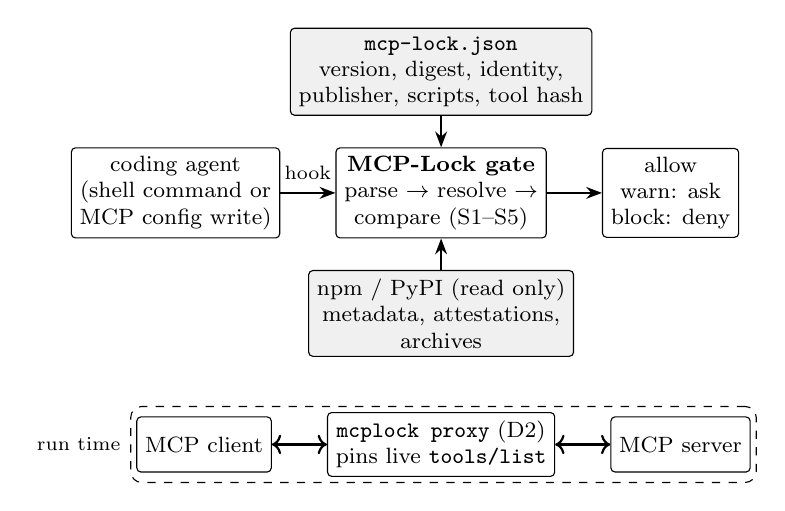
\begin{tikzpicture}[font=\footnotesize, node distance=4mm and 7mm,
  box/.style={draw, rounded corners=1.5pt, align=center, inner sep=3pt, minimum height=7mm},
  data/.style={box, fill=black!6},
  arr/.style={-{Stealth[length=2mm]}, thick}]
\node[box] (agent) {coding agent\\(shell command or\\MCP config write)};
\node[box, right=of agent, minimum width=2.6cm] (gate) {\textbf{MCP-Lock gate}\\parse $\rightarrow$ resolve $\rightarrow$\\compare (S1--S5)};
\node[data, above=of gate] (lock) {\code{mcp-lock.json}\\version, digest, identity,\\publisher, scripts, tool hash};
\node[data, below=of gate] (reg) {npm / PyPI (read only)\\metadata, attestations,\\archives};
\node[box, right=of gate, minimum width=1.4cm] (dec) {allow\\warn: ask\\block: deny};
\node[box, below=7mm of reg, minimum width=2.6cm] (proxy) {\code{mcplock proxy} (D2)\\pins live \code{tools/list}};
\node[box, left=of proxy] (client) {MCP client};
\node[box, right=of proxy] (server) {MCP server};
\draw[arr] (agent) -- node[above, font=\scriptsize, yshift=1pt]{hook} (gate);
\draw[arr] (lock) -- (gate);
\draw[arr] (reg) -- (gate);
\draw[arr] (gate) -- (dec);
\draw[arr, <->] (client) -- (proxy);
\draw[arr, <->] (proxy) -- (server);
\node[draw, dashed, rounded corners, fit=(client)(proxy)(server), inner sep=2pt, label={[font=\scriptsize]left:run time}] {};
\end{tikzpicture}
\caption{MCP-Lock. Before launch, the gate compares what a command would fetch with the lock and never runs package
code. At run time, the optional proxy (hardening D2) checks every tool listing against a pin.}
\label{fig:arch}
\end{figure}

\textbf{Gate.} Before a command runs, the gate parses it (installs and runner launches, including \code{npx},
\code{pnpm dlx}, \code{bunx}, \code{uvx}, \code{pipx run}), resolves what the launch would fetch now, and compares it with
the lock entry. It reads registry metadata, attestations and archives, and never executes package code.
Fig.~\ref{fig:arch} shows the flow and Table~\ref{tab:signals} lists the signals; S1 is our reimplementation of the Bagmar and Saraf checks~\cite{bagmar2026setup}.
A block denies the command; a warning asks the user. The gate runs as a Claude Code \code{PreToolUse} hook on shell
commands and on writes to MCP configuration files, and fails closed to ``ask'' on internal errors.

\begin{table}[t]
\caption{Gate signals. S2--S5 compare a launch against its lock entry.}
\label{tab:signals}
\centering\footnotesize
\begin{tabular}{@{}lp{4.6cm}l@{}}
\toprule
Signal & Fires when & Action \\
\midrule
S1 & name confusable, absent or younger than 30 days; untrusted source; hidden index; known-vulnerable pin & block \\
S2 & provenance disappears, or a different repository / workflow / builder built the new version & block \\
S3 & npm: published by hand after CI releases, or by a non-maintainer & warn \\
S4 & new install-time lifecycle script (PyPI: sdist-only release after wheels) & block \\
S5 & canonical tool hash differs (diff shown) & warn \\
gate & server not locked / same version, different digest & warn / block \\
\bottomrule
\end{tabular}
\end{table}

% ------------------------------------------------------------------------------------------------
\section{RQ2: Pre-Registered Evaluation}
\label{sec:eval}
\textbf{Design.} Hypotheses, corpora, scoring and a kill rule were registered on OSF~\cite{osf2026prereg} before any scored run, with the
gate frozen at a tagged commit. \textbf{H1:} on real attacks, \G{} (S1--S5) detects more cases than \SC{}, the stronger
reading of the baseline. \textbf{H2:} on benign upgrades, \G{}'s false-block rate differs from \SC{}'s. \textbf{Kill
rule:} the method claim is withdrawn if S2--S5 add fewer than two detections while \G{}'s false-block rate is equal or
worse. Detection is block or warn; H1 and H2 use exact McNemar tests~\cite{mcnemar1947} with Holm
correction~\cite{holm1979}; proportions carry Wilson 95\% intervals~\cite{wilson1927}. Six deviations, all logged before
the affected results, concern replay mechanics and corpus construction.

\textbf{Corpora.} R-B: \NRB{} scenarios of the baseline paper. R-M: \NRM{} real malicious npm/PyPI versions from OpenSSF and
Datadog reports~\cite{ossfmalicious,datadogmalicious}, \NRMC{} hijacked existing packages (class C, locked at the last
clean version) and \NRMN{} new or typosquatted ones (class N). R $=$ R-B $\cup$ R-M, $n = \NR$. R-S: synthetic rug
pulls on a local registry (four classes $\times$ 10 servers, 10 controls), reported separately. B: \NB{} benign upgrades
(\NBMcp{} MCP, the census transitions of Section~\ref{sec:census}; \NBNpmTop{} top npm; \NBPyTop{} top PyPI). Every
case is replayed offline as of its publication time; malicious archives are only read, never executed.

\begin{table}[t]
\caption{Confirmatory results (Wilson 95\% CIs).}
\label{tab:rq2}
\centering\footnotesize
\begin{tabular}{@{}lll@{}}
\toprule
 & \SC & \G \\
\midrule
Detection on R & \DetSCP{} \DetSCCI & \DetGP{} \DetGCI \\
\quad block only & \DetSCBlockP{} \DetSCBlockCI & \DetGBlockP{} \DetGBlockCI \\
False blocks on B & \FbSCP{} \FbSCCI & \FbGP{} \FbGCI \\
Warnings on B & 0 & \WarnGP{} \WarnGCI \\
\midrule
H1 & \multicolumn{2}{p{5.1cm}}{\AddedDet{} \G-only vs.\ \SCOnly{} \SC-only cases; exact McNemar $p = \McNemarHOne$
(Holm $\HolmHOne$)} \\
H2 & \multicolumn{2}{p{5.1cm}}{false blocks +\FbDiffPP{} pp \FbDiffCI; $p = \McNemarHTwo$} \\
Kill rule & \multicolumn{2}{p{5.1cm}}{\AddedDet{} added detections $\ge 2$: not killed} \\
\bottomrule
\end{tabular}
\end{table}

\textbf{Results.} Table~\ref{tab:rq2} gives the confirmatory results. H1 holds: \G{} detects more real attacks. H2
holds in the unfavourable direction: \G's false-block rate is \FbDiffPP{} percentage points higher than \SC's, a small
but significant cost. The kill rule is not triggered. Counting only blocks, which do not depend on a user reading a
warning, barely changes detection (\DetGBlockP{} vs.\ \DetSCBlockP). In the ablation, removing S4 loses \AblFour{} of \G's detections, removing S5 \AblFive, S3 \AblThree{}
and S2 \AblTwo. On hijacked packages (class C) \G{} detects \RMCGP{} \RMCGCI{} against
\RMCSCP{} for \SC, mostly install scripts added by the 2025 worm campaigns~\cite{cisa2025shaihulud,checkpoint2025shaihulud}. By
publication date, \WaveOneOnly{} and \WaveTwoOnly{} of the \AddedDet{} added detections fall in the two Shai-Hulud
waves (14--30 Sep.\ and 21 Nov.--5 Dec.\ 2025). Outside both windows the gain remains: \G{} detects \OutGP{} of
\OutN{} R-M cases against \OutSCP{} for \SC{} (\OutOnly{} vs.\ \OutSCOnly{} discordant cases, $p = \OutMcNemar$;
exploratory). On new names (class
N) both detect \RMNGP{} through the baseline's age rule. Provenance continuity (S2) added nothing on real attacks
because removed malicious versions leave no registry record, so S2 and S3 were evaluable on only
\EvalSTwo{} of \NRM{} R-M cases, and only \STwoRMCP{} of class-C locks had provenance to begin with.

On the synthetic rug pulls, \G{} detects \RSG{} and \SC{} \RSSC; S5 alone carries the two tool-definition classes, S4 the
install-script class, and S2 and S3 each catch the stolen-token class. No control was flagged (\RSCtrl).

The cost is paid in reviews. \G's false blocks barely move (\FbExtra{} more than \SC), but S5 adds warnings on
\WarnGP{} of benign upgrades, essentially all in the MCP stratum, where honest servers change tools often (RQ1). Per
added detection, \G{} costs \FbPerDet{} extra false blocks and \WarnPerDet{} extra warnings. The baseline's own
\FbSCP{} false-block rate comes from its 30-day age rule replayed at upgrade time (\FbSCMcpP{} of MCP upgrades).
Median gate latency is \LatColdMed{}\,s on a cold cache (p95 \LatColdPNF{}\,s; $n = \LatN$) and \LatWarmMed{}\,s warm.

\textbf{Age-rule sensitivity (exploratory).} Almost all of \G's false blocks come from S1's 30-day age rule, which
guards the first use of a name but fires again on every upgrade of a young server that the user has already locked.
Waiving it for locked servers, and changing nothing else, lowers \G's false blocks on B from \FbGP{} to \AgeFbP{}
\AgeFbCI. Interruptions (block or warn) fall from \InterGP{} to \AgeInterP; warnings rise to \AgeWarnP, because some former
blocks also carried a tool-drift warning, which now surfaces on its own. Detection on R drops by \AgeLost{} hijacked packages that were young
enough for the age rule to catch, to \AgeDetP{} (\AgeDet), still \AgeAdded{} more than \SC. This was not
pre-registered; the confirmatory results above are unchanged.

% ------------------------------------------------------------------------------------------------
\section{RQ3: Adaptive Attacker}
\label{sec:adaptive}
\textbf{Setup.} For each tier we built the cheapest attack we could find against a gate whose checks, lock format and
parser are known, as \ENCases{} packages on a local registry with inert payloads, plus \EElevenN{} command-line variants of one
attack (Table~\ref{tab:matrix}). All runs use the frozen gate; nothing was published publicly or executed.

\begin{table}[t]
\caption{Evasion matrix. \G: frozen gate; D: all hardening switches D1--D5. E11 counts detected command shapes.}
\label{tab:matrix}
\centering\footnotesize
\begin{tabular}{@{}llp{3.55cm}ll@{}}
\toprule
Case & Tier & Attack & \G & D \\
\midrule
E1 & T1 & new name, edit distance $\ge 2$, older than 30 days & warn & warn \\
E2 & T2 & stolen token; lock has no provenance & allow & block \\
E3 & T2 & stolen token; lock has provenance & block & block \\
E4 & T3 & payload via the genuine release workflow & allow & allow \\
E5 & T4 & poisoned description built at run time & warn & block \\
E6a/b & T4 & tools fetched from a URL; new / no new version & allow & block \\
E7 & T4 & poison in an input-schema field description & warn & block \\
E8a/b & T4 & time-bomb tool / tool from a base64 blob & warn/allow & block \\
E9 & T5 & payload and tools in a caret-range dependency & allow & block \\
E10 & T2/T4 & extra file added to a locked PyPI release & allow & block \\
E11 & any & \EElevenN{} command shapes (detected) & \EElevenG/\EElevenN & \EElevenH/\EElevenN \\
\bottomrule
\end{tabular}
\end{table}

\textbf{What evades.} The frozen gate blocks \EGBlock{} and warns on \EGWarn{} of the \ENCases{} attacks; \EGAllow{}
pass. Static extraction cannot see tools built at run time or fetched from a URL (E6, E8b),
and a rug pull through a remote file needs no new version at all (E6b). Locking the top-level archive leaves
dependencies free to move (E9). A stolen token defeats S2 and S3 whenever the lock never had provenance (E2), and the
same-version check compares only the locked file (E10). Commands hidden behind \code{npm exec}, \code{sh -c} or a shell
variable escape the parser. The conditions these attacks need are common: \ExpNoProvP{} of benign locks have no provenance (E2),
\ExpNonStaticP{} of versions hide their tools from static extraction (E6/E8), and \ExpFloatSdkP{} of npm servers
float their MCP SDK dependency (E9, a lower bound that counts one dependency). A payload shipped through the genuine
release pipeline (E4) carries genuine provenance; no lock can tell it apart from an honest release.

\textbf{Hardening (exploratory).} We implemented five switches, off by default; with all off the gate is the frozen
code, and a re-replay of every Phase-4 corpus is identical case by case. \emph{D1} locks the resolved npm dependency
tree and applies the S2--S4 rules to every dependency whose version changed. \emph{D2} is a stdio proxy that pins the
live \code{tools/list} per tool (trust on first use), rejects listings that add or change a tool, and refuses calls to
unpinned tools; it checks every listing, so a time bomb is caught when it fires; this is the design of existing
runtime pinning tools~\cite{mcppin,mcpseal}, measured here. \emph{D3} locks every file of a PyPI
release. \emph{D4} requires provenance. \emph{D5} normalises the evasive command shapes. With all five, \EAllBlock{} of
\ENCases{} attacks block and \EElevenH{} of \EElevenN{} command shapes are caught; E1 still only warns and E4 passes.

\begin{figure}[t]
\centering
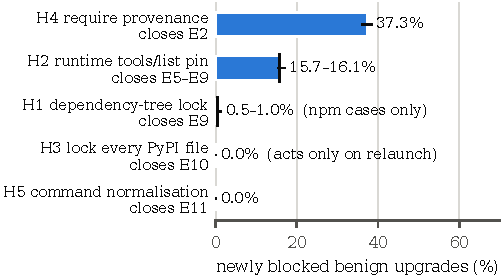
\includegraphics[width=\columnwidth]{figures/hardening_cost.pdf}
\caption{Cost of each hardening switch: benign upgrades it would newly block on top of the frozen gate (bar: upper
estimate with Wilson 95\% CI; tick: lower estimate). D1 is measured on the \HOneN{} npm upgrades, D3 on PyPI.}
\label{fig:cost}
\end{figure}

\textbf{Cost.} Figure~\ref{fig:cost} shows the cost of each switch. D3 and D5 cost nothing on benign upgrades:
D5 changes no decision (\HFive), and D3 only acts when the locked version is relaunched, which no upgrade does; as an
exposure measure, \HThreeLateP{} of locked PyPI releases later gained a file. D1 adds blocks to
\HOneBlockLateP--\HOneBlockEarlyP{} of npm upgrades, depending on whether the lock was taken just before the upgrade or
when the old version was released. A strict tree lock that blocks every dependency change, as \code{npm ci} would,
blocks \HOneStrictLateP--\HOneStrictEarlyP{} instead; applying continuity rules to dependencies, instead of
pinning them exactly, is what keeps the tree lock usable. D2 and D4 are expensive: D2 newly blocks \HTwoAddLoP--\HTwoAddHiP{} of benign upgrades, all
MCP servers that changed tools, and D4 \HFourAddP. The live tool list of a historical version cannot be observed without
running it, so D2's benign cost assumes it equals the static extraction, and the \HTwoUnmeas{} upgrades without
statically visible tools are counted as costless.

\textbf{Safer alternatives (exploratory).} A block tells the agent what not to run but not what to run instead, so an
agent may retry with something worse. When the gate flags a command, it now proposes a replacement and shows it only if
the gate itself passes the rewritten command; the decision is never changed. For a locked server it suggests the newest
version between the lock and the target that passes every lock check, falling back to the locked version; for a
typosquat, the popular package the name imitates; for a vulnerable pin, the lowest release with no advisory, stepping
forward when a fix carries advisories of its own. The Claude Code hook appends the suggestion to its deny reason, so the
agent can retry with it. A verified suggestion is offered for \SgRMCCov{} real hijacked versions (class C), \SgRSCov{}
synthetic rug pulls and \SgADVCov{} flagged adaptive attacks. Every one of them is the locked version, and none is the
malicious version (\SgRMCBad{} for class C, 95\% CI \SgRMCBadCI). For R-B it names the intended package in
\SgRBName{} typosquat scenarios and a fixed release for \SgRBVer{} vulnerable pins. It stays silent on all \SgRMNFlag{}
newly registered malicious names, none of which is within edit distance~2 of a popular package. Class C correctness
holds by construction, since the lock is the last version no advisory lists. On benign upgrades the
suggestion is always a rollback to the reviewed version (\SgBCov), which is safe but defers an honest update until the
user re-locks. Suggesting a typosquat's target or a fixed version is existing practice (e.g.\ \code{npm audit fix}); here
every suggestion, including the rollback, is checked by the gate before the agent sees it.

% ------------------------------------------------------------------------------------------------
\section{Discussion and Limitations}
\textbf{What the evidence supports.} Pinning catches real attacks that the name-and-source checks miss, but the
confirmed gain is an install-script diff (S4), a classic supply-chain signal rather than an MCP-specific one. A deployable
gate should not re-apply first-use checks to servers already in the lock: doing so is what made both gates block a third
of honest upgrades. Tool pinning (S5) is what catches MCP rug pulls, and it is necessary because metadata signals do not accompany tool changes (RQ1),
yet it warns on \WarnGMcpP{} of honest MCP upgrades. Of these \SfiveWarnN{} warnings, \SfDescP{} change a
description, \SfAddsP{} add a tool, \SfSchemaP{} change only an input schema and \SfRemoveP{} only remove tools
(exploratory). The first three are what a rug pull changes, so S5 cannot be narrowed without losing the attacks it
exists for. The \SfRealAlone{} real attacks that S5 alone detects both report removed tools; no case in R is a
known tool-definition rug pull, so S5's value against that attack rests on R-S and the adaptive cases. Provenance continuity is sound but rarely applicable: most
packages have none, and attackers who remove their versions take the evidence with them.

\textbf{Simpler alternatives (exploratory).} Two steps need no gate. Pinning the exact version in the MCP
configuration prevents every class-C case (\PinRM{} of R-M) but holds back all \NB{} benign upgrades until the user
edits the configuration. npm's \code{-{}-ignore-scripts} keeps the install-time code of up to \IgnRMP{} of npm R-M
cases from running (an upper bound, since a payload may also run at launch) and skips an honest install script in
\IgnBP{} of npm upgrades. Together with the baseline hook it covers \SCIgnP{} of npm R-M cases, about as many as
\G{} (\GNpmP), so on real attacks most of \G's gain is available more cheaply. What \G{} adds is continuity of
tool definitions and provenance, which the real attacks barely exercised, unattended upgrades when nothing changed,
and a diff to review when something did.

\textbf{Limits of a lock.} Every lock in this paper trusts the state at lock time and flags change. An attacker in the
release pipeline (T3) produces change that is indistinguishable from an honest release, and a runtime pin can only
compare against what was trusted first. Reviewing the diff remains the user's job; the gate makes the diff visible.

\textbf{Threats to validity.} Static extraction under-counts tools (recall \ValRec{}), so drift and S5 coverage are lower
bounds. R-M contains only attacks that were caught and reported; attacks still undetected are absent by definition.
Replay reconstructs metadata as of each case's time but cannot recover removed versions, which is why S2/S3 evaluability
is low. Class C follows a mechanical rule (an earlier clean version exists) and may include attacker-owned packages with
a benign first release. The adaptive attacks were built by the authors of the defence; the hardening results are
exploratory and were not pre-registered, as are the safer-alternative suggestions and the publication-window split. D2's matrix verdicts use live tool
lists written down from each attack's source; running the \RtCases{} locked servers in containers with no outside network gave
the same D2 verdict in \RtAgree{} cases and the same findings in \RtSame, with E8a's clock set past its trigger date. Time of lock is unknown in practice, which is why D1 is reported as a
range.

% ------------------------------------------------------------------------------------------------
\section{Related Work}
\textbf{MCP security.} Surveys and taxonomies describe tool poisoning, rug pulls and malicious
servers~\cite{hou2025mcp,zhao2025attack}, and practitioners described the rug-pull pattern early on~\cite{invariant2025poisoning}.
Hasan et al.\ analyse the security and maintainability of open-source servers~\cite{hasan2025glance}. Closest to RQ1,
Kraishan measures drift of the fields the MCP registry versions (descriptions, packages, endpoints) across 8,900
multi-version servers and notes that tool definitions are not versioned there~\cite{kraishan2026drift}; we measure the
tool definitions themselves from package archives, and build the client-side pinning that work recommends. Metere
proposes signed admission and per-server tool allowlists for remote servers~\cite{metere2026attested}, and ETDI signed,
versioned tool definitions~\cite{bhatt2025etdi}; MCP-Lock instead needs no change to servers or registries.

\textbf{Tool pinning.} Pinning tool definitions is established practice. MCP-Scan hashes tool descriptions to detect
rug pulls~\cite{invariant2025mcpscan}, and open-source proxies pin each tool's definition in a committed lockfile and
block a changed listing; one also records the package version and registry digest~\cite{mcppin,mcpseal}. These tools
start the server to read its tools. MCP-Lock's S5 reads them from the archive before launch, combines them with
provenance, publisher and install-script continuity, and is evaluated on real attacks and benign upgrades; our runtime
proxy (D2) follows the existing design.

\textbf{Agent supply chains.} Bagmar and Saraf weaponise setup instructions against coding agents and propose the
pre-install hook we use as baseline~\cite{bagmar2026setup}. Kapner et al.\ scan agent configurations and report unpinned
MCP declarations~\cite{kapner2026harness}. Shan finds in a pre-registered audit that coding assistants almost never
check trust signals before installing~\cite{shan2026check}, which motivates a gate that checks on their behalf.

\textbf{Package supply chains.} Attack catalogues~\cite{ohm2020backstabber,ladisa2023sok} and ecosystem
studies~\cite{zimmermann2019small,zahan2022weak} document account takeover and install-script abuse, the patterns behind
S3 and S4. Sigstore~\cite{newman2022sigstore}, SLSA~\cite{slsa2023provenance} and PEP~740~\cite{pep740} make build
identity verifiable; MCP-Lock uses that identity for continuity rather than for absolute trust.

% ------------------------------------------------------------------------------------------------
\section{Conclusion}
MCP servers change the tools they present to models often, and nothing in their metadata says so. A lock that pins
archive, provenance, publisher, install scripts and tool definitions catches \AddedDet{} real attacks that the existing
gate misses, at a cost paid mostly in reviews of honest tool changes; on npm, the existing gate with
\code{-{}-ignore-scripts} covers about as many. Against an adaptive attacker, the frozen gate
blocks \EGBlock{} and warns on \EGWarn{} of \ENCases{} attacks; dependency-tree locking, runtime tool pinning, file-level PyPI locking and command
normalisation close most of the rest, and we measure what each costs. Two gaps remain open for any lock-based
defence: attacks shipped through the legitimate release pipeline, and the review fatigue of honest change.

\section{Artifact Availability}
\label{sec:artifact}
Code, lockfile specification, replay bundles, results and logs:
\url{https://github.com/ftaakash/MCP-Lock}. Pre-registration: \url{https://osf.io/2amj3}, DOI 10.17605/OSF.IO/2AMJ3. Every number in this paper is
generated from the result files by \code{paper/make\_numbers.py}.

\bibliographystyle{IEEEtran}
\bibliography{refs}

\end{document}
